\documentclass[crop,tikz]{standalone}

\usetikzlibrary{
	chains,
	positioning,
	arrows.meta,
	decorations.pathreplacing,
	calc,
	fit,
	shapes.geometric
}

\begin{document}

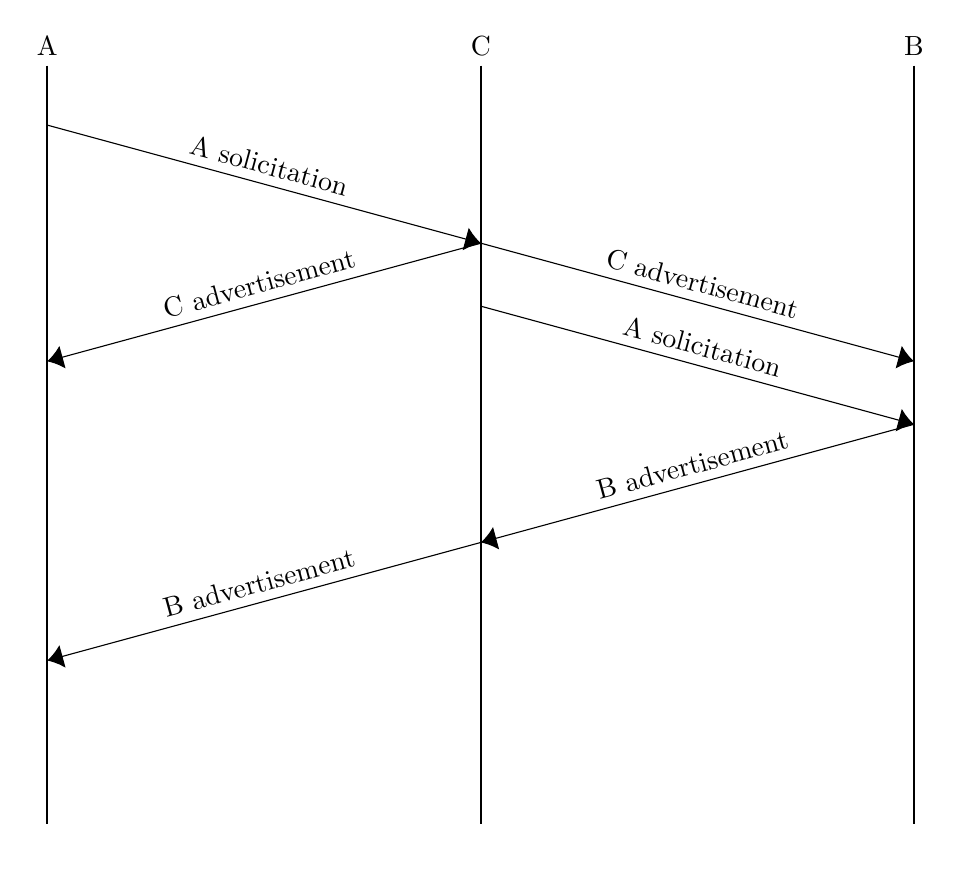
\begin{tikzpicture}[node distance=5cm,auto]
	\node[] (c) {C};
	\node[right = of c] (b) {B};
	\node[left = of c] (a) {A};
	\node[below of=c, node distance=10cm] (c_ground) {};
	\node[below of=b, node distance=10cm] (b_ground) {};
	\node[below of=a, node distance=10cm] (a_ground) {};

	\draw[thick] (c) -- (c_ground);
	\draw[thick] (b) -- (b_ground);
	\draw[thick] (a) -- (a_ground);

	\draw[-{Latex[length=2mm,width=3mm]}] ($(a)!0.1!(a_ground)$) -- node[above,sloped]{A solicitation}  ($(c)!0.25!(c_ground)$);

	\draw[-{Latex[length=2mm,width=3mm]}] ($(c)!0.25!(c_ground)$) -- node[above,sloped]{C advertisement} ($(b)!0.4!(b_ground)$);
	\draw[-{Latex[length=2mm,width=3mm]}] ($(c)!0.25!(c_ground)$) -- node[above,sloped]{C advertisement} ($(a)!0.4!(a_ground)$);

	\draw[-{Latex[length=2mm,width=3mm]}] ($(c)!0.33!(c_ground)$) -- node[above,sloped]{A solicitation} ($(b)!0.48!(b_ground)$);

	\draw[-{Latex[length=2mm,width=3mm]}] ($(b)!0.48!(b_ground)$) -- node[above,sloped]{B advertisement} ($(c)!0.63!(c_ground)$);
	\draw[-{Latex[length=2mm,width=3mm]}] ($(c)!0.63!(c_ground)$) -- node[above,sloped]{B advertisement} ($(a)!0.78!(a_ground)$);

	\end{tikzpicture}

\end{document}